\chead{\textit{Results}}  				
\section{Results}
\label{sec:res}

The following chapter presents the results of this thesis. First, a case study system is presented as a reference example to calculate both the centralized and decentralized problems. Next, the convergence of the decentralized algorithm is analyzed, and several issues are presented that influence the algorithm's convergence rate. Following this, the results of both approaches are compared against each other.

\subsection{Case Study System}
\label{sec:res:tns}

This section describes the \gls{tns} that is used as a case study system to examine the decentralized optimal power flow implementation. The system is rather simple to grasp the findings better. The implementation of the \gls{tns} can be found in the file \path{src/cases/three_node.jl}. As mentioned in section \ref{sec:app:implementation}, the source code can be easily extended by a more detailed case study system. The \gls{tns} consists of three nodes. A different set of generators and storages is located at each of them. Each node has a different two-period demand vector. A total of three transmission lines connect the nodes. Thus, every node has two neighbors. All network elements must meet the requirements described in section (\ref{sec:app:mod-framework}). The network layout and the corresponding parameters of the elements are shown in figure (\ref{fig:tns}).

\begin{figure}[h]
	\centering
	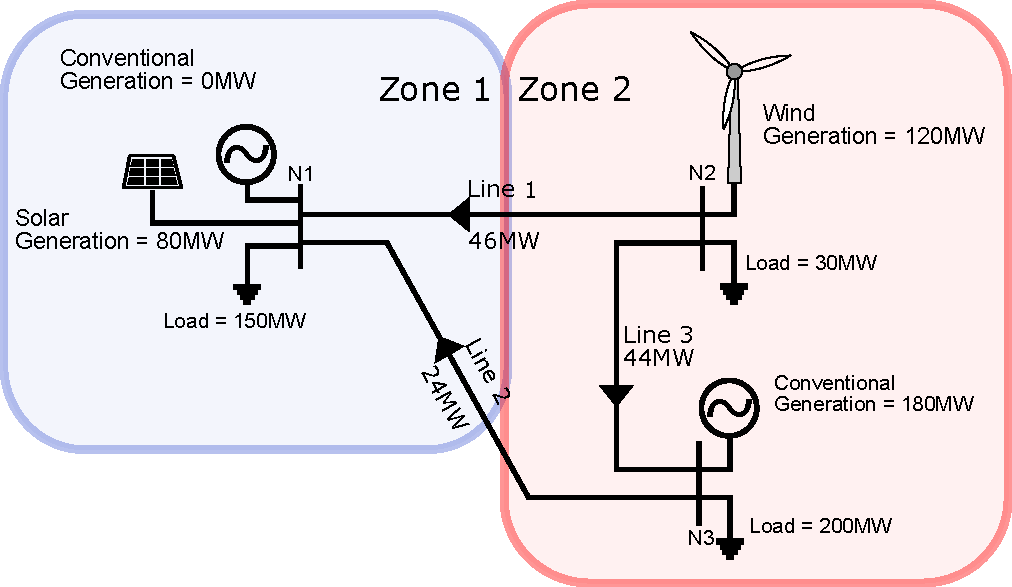
\includegraphics[width=\textwidth]{three-node-system.png}
	\caption{Three Node System Case Study System}
	\label{fig:tns}
\end{figure}

There is a total of four generators in the system. The name of the generators refers to real-life power plants. For example, at node 3 (N3), the coal generator has the largest production capacity and is more expensive than the photovoltaic and wind generator. On the other hand, the gas generator has the highest marginal costs in the system to account for a generator that is only used to cover peak loads. The marginal costs for the renewable generators are not set to zero because this would violate the penalty terms of the decentralized formulation. The marginal costs of these generators are set to 3 and 4, respectively. Both renewable generators act like a dispatchable unit in the \gls{tns}. This contradicts the nature of renewable energy resources. However, compared to the other generators, the marginal costs of the photovoltaic and wind generator are minimal. Thus, these generators will always be dispatched.

\begin{table}[h!]
    \centering
    \begin{tabular}{lrr}
        Generators $\set{G}$ & $mc$ [EUR/MWh] & $\overline{p}$ [MW] \\ \toprule
        PV & 3 & 80 \\
        Wind & 4 & 120 \\
        Coal & 30 & 300 \\
        Gas & 50 & 120 \\
        \bottomrule
    \end{tabular}
    \caption{Generator parameters for the Three Node System} \label{tab:res:param-gen}
\end{table}

In addition to the generators, there is one storage in the \gls{tns} that is located at node 1. This network element has the cheapest marginal costs to ensure that the storage is favored in all dispatch decisions. Also, the total system demand of time step one is set to $180 MW$ and thus smaller than the capacity of the photovoltaic and wind generator together. Subsequently, the storage should be charged to reduce the power output of either the coal or gas generator in time step two. The parameters of the storage are shown in table \ref{tab:res:param-stor}.


 \begin{table}[h!]
    \centering
    \begin{tabular}{lrrr}
        Storages $\set{S}$ & $mc$ [EUR/MWh] & $\overline{p}$ [MW] & $\overline{e}$ [MWh] \\ \toprule
        Battery & 1 & 10 & 20 \\
        \bottomrule
    \end{tabular}
    \caption{Storage parameters for the Three Node System} \label{tab:res:param-stor}
\end{table}

Lastly, the capacities of the transmission lines are set to values so that a congestion on either one line is almost certain. All transmission line specific parameters can be found in table \ref{tab:res:param-line}.

 \begin{table}[h!]
    \centering
    \begin{tabular}{lrr}
        Transmission Lines $\set{L}$ & $f$ [MWh] & $S$ [1/$\Omega$] \\ \toprule
        Line 1 & 20 & 1 \\
        Line 2 & 45 & 1 \\
        Line 3 & 70 & 2 \\
        \bottomrule
    \end{tabular}
    \caption{Transmission line parameters for the Three Node System}
    \label{tab:res:param-line}
\end{table}

\subsection{Convergence Analysis of the Decentralized Algorithm}

The following section studies the convergence of the decentralized algorithm. As already mentioned, several convergence problems were faced while implementing the mathematical formulations from section \ref{sec:app:dom} with Julia. \\

\begin{figure}[h!]
	\centering
	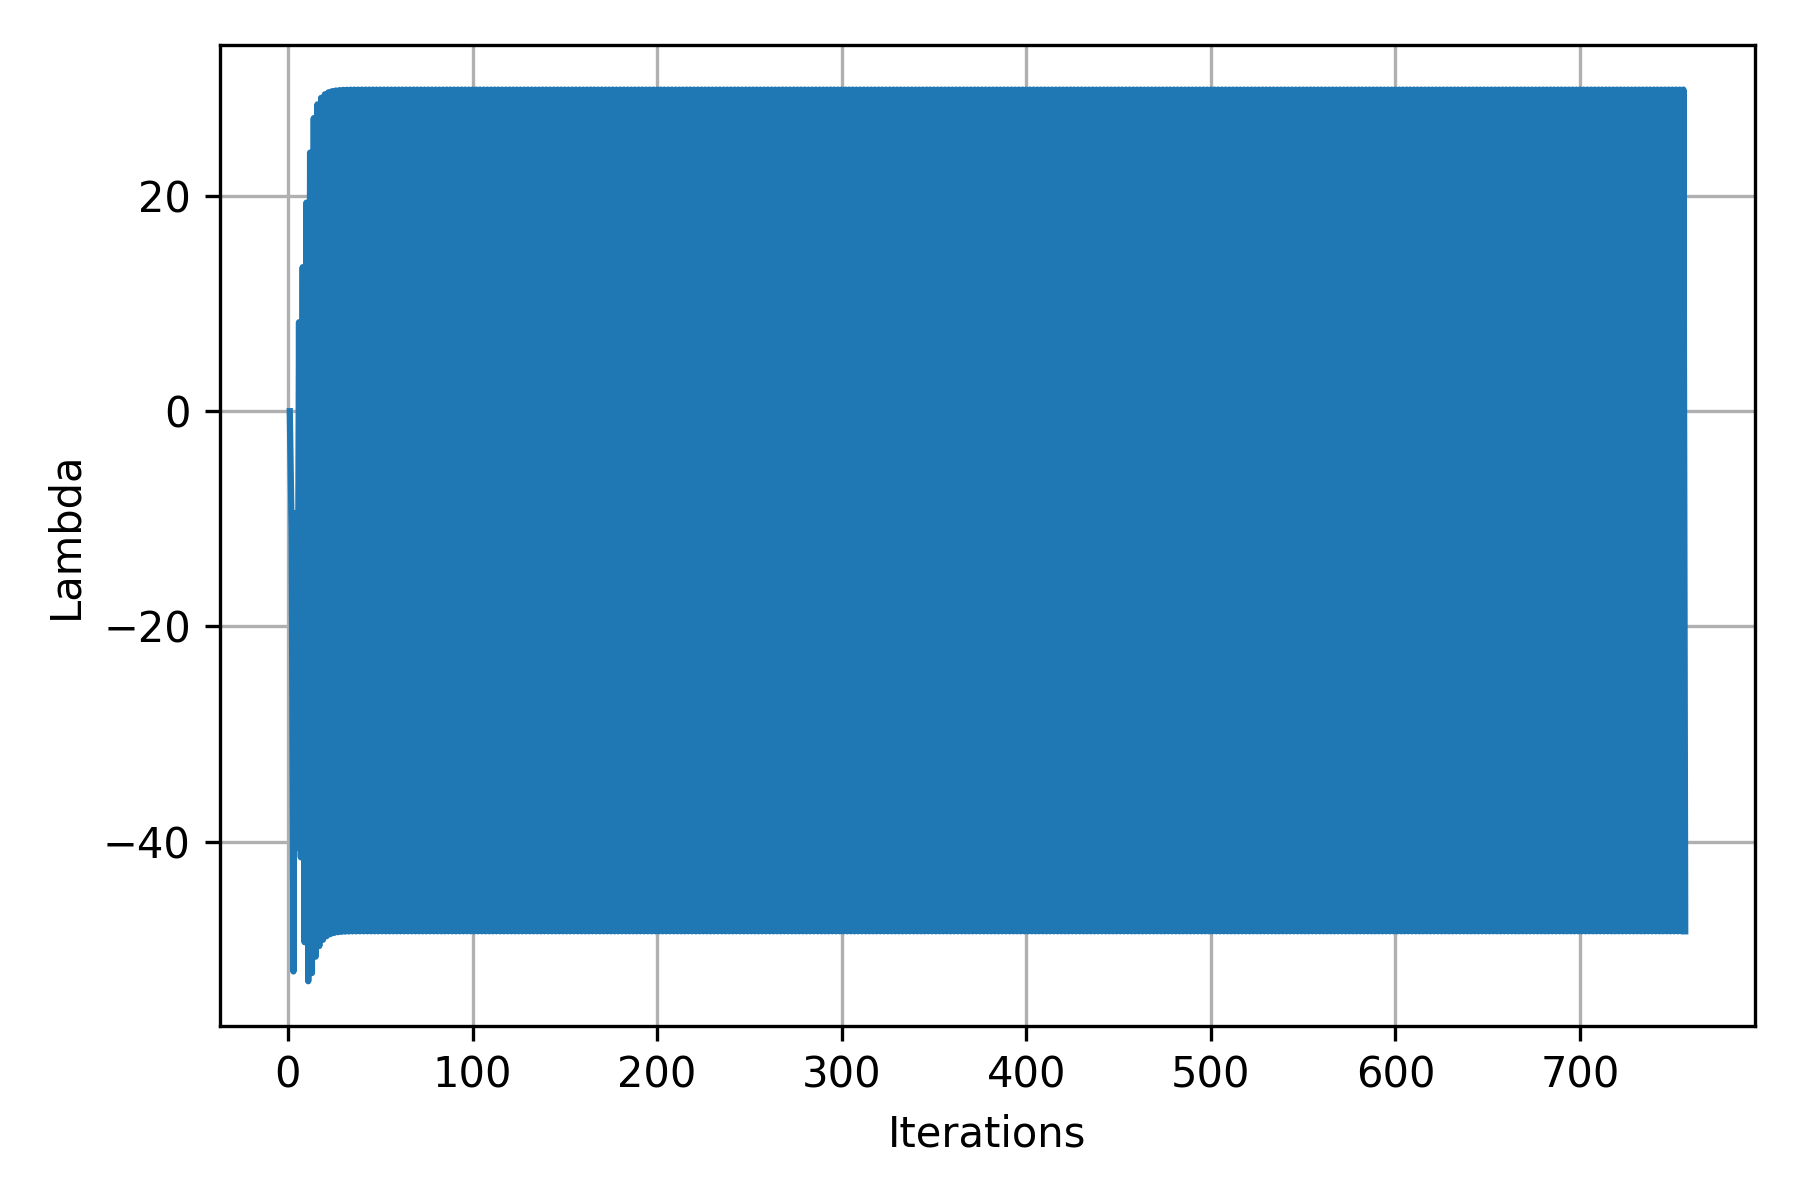
\includegraphics[width=0.8\textwidth]{plots/big_gamma_lambda_t1.png}
	\caption{Convergence Problem I: Damping parameter too large}
	\label{fig:conv-problem-1}
\end{figure}

\begin{figure}[h!]
	\centering
	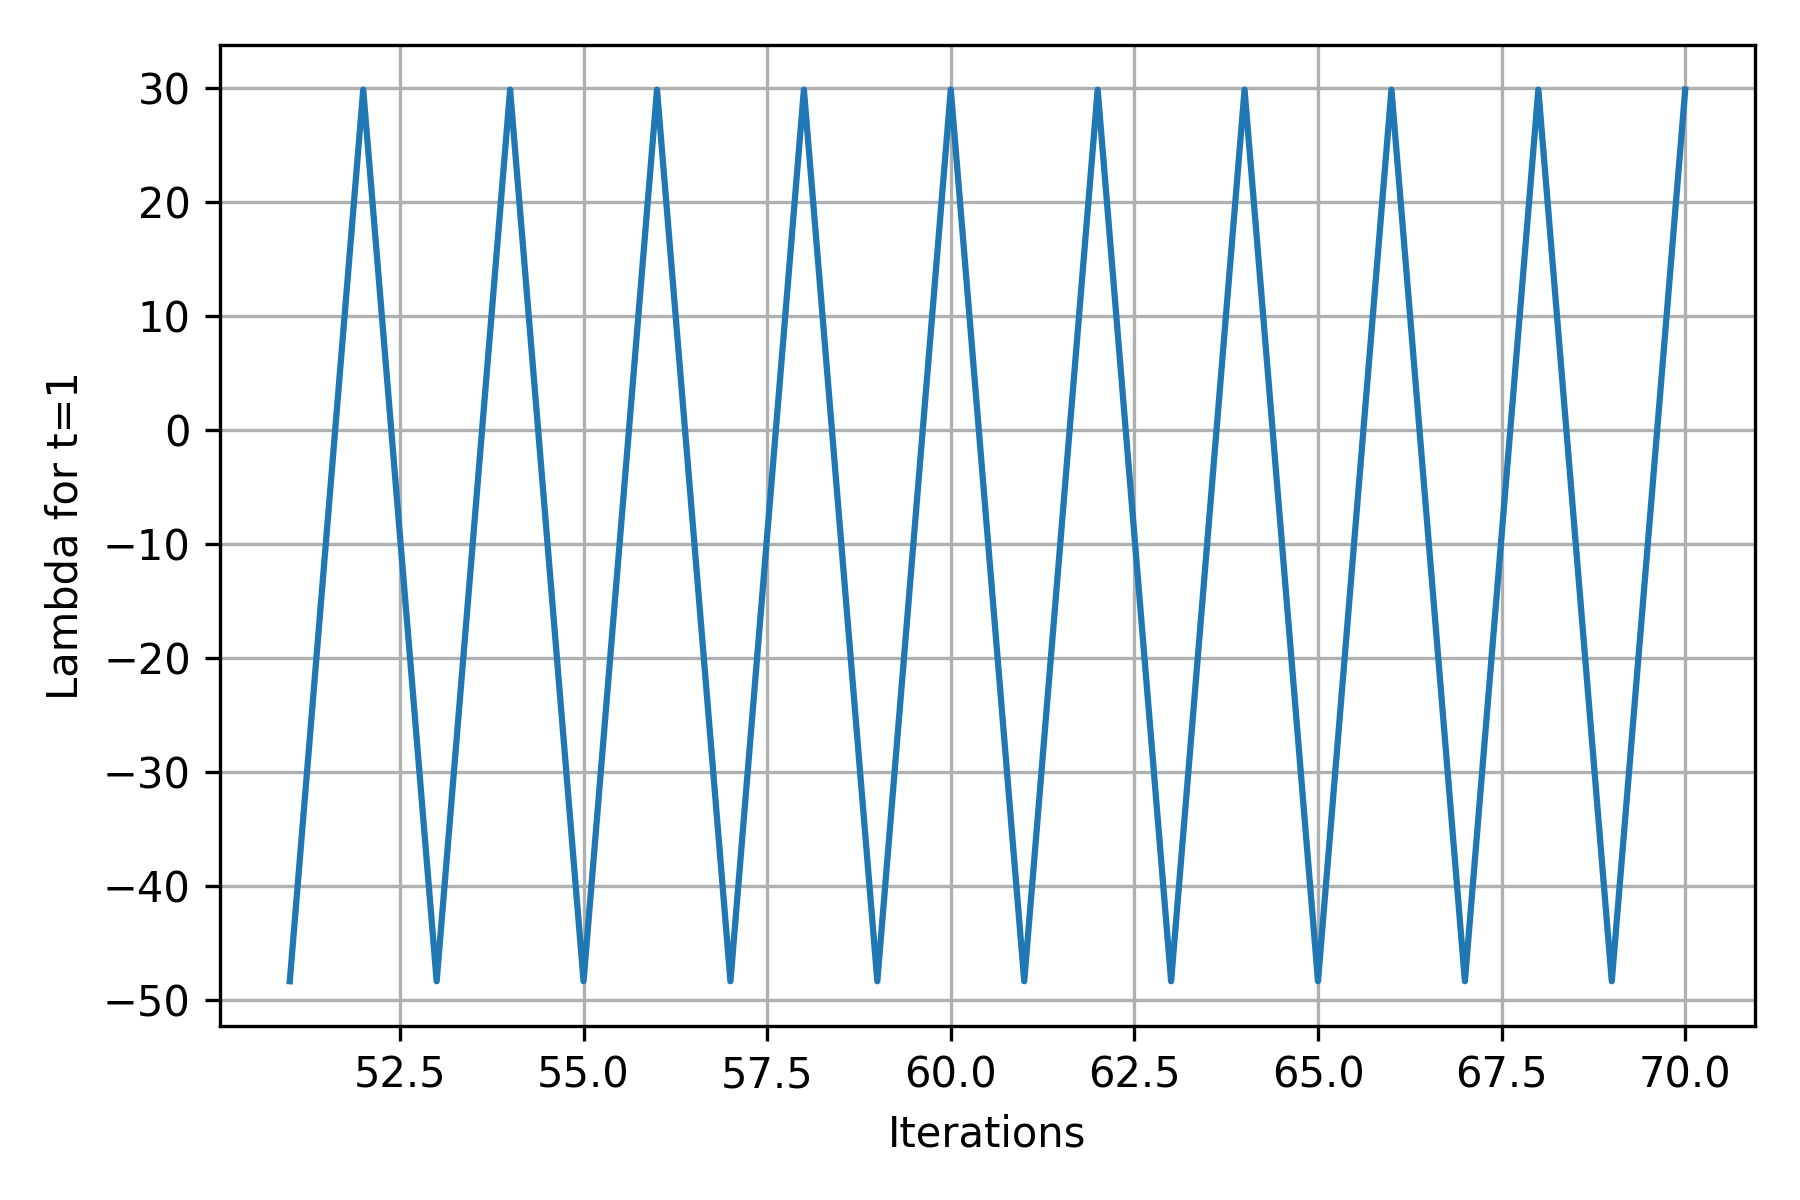
\includegraphics[width=0.8\textwidth]{plots/big_gamma_lambda_t1_i_50-70.png}
	\caption{Convergence Problem I: Zoomed version of figure (\ref{fig:conv-problem-1})}
	\label{fig:conv-problem-1-zoom}
\end{figure}

First of all, it was found that the algorithm is susceptible to the damping parameter $\gamma$. Although stated as one of the main advantages of the \gls{admm} that one has to choose only one parameter, finding the correct value for the damping parameter represented a challenge. In figure (\ref{fig:conv-problem-1}) one can see the iteration values for the dual variable $\lambda_1$ for time step one. The value of $\lambda_1$ is plotted for every iteration. The damping parameter was set to $\gamma = 0.5$. As one can see, the decentralized algorithm did not converge and was interrupted after 650 iterations. The values for $\lambda_1$ seemed to be jumping between 30 and -48. See also figure (\ref{fig:conv-problem-1-zoom}) for a better visualization of the divergence. Different plotting scripts were defined in \path{src/helpers/plotting.jl} to better zoom and pan the plots. After analyzing the plots, it could be identified that the damping parameter was too large. Decreasing the damping parameter to $\gamma = 0.3$ solved the divergence problem of the dual variable $\lambda_t$. Figure (\ref{fig:conv-lambda}) shows the convergence plot of $\lambda_1$. \\

\begin{figure}[h!]
	\centering
	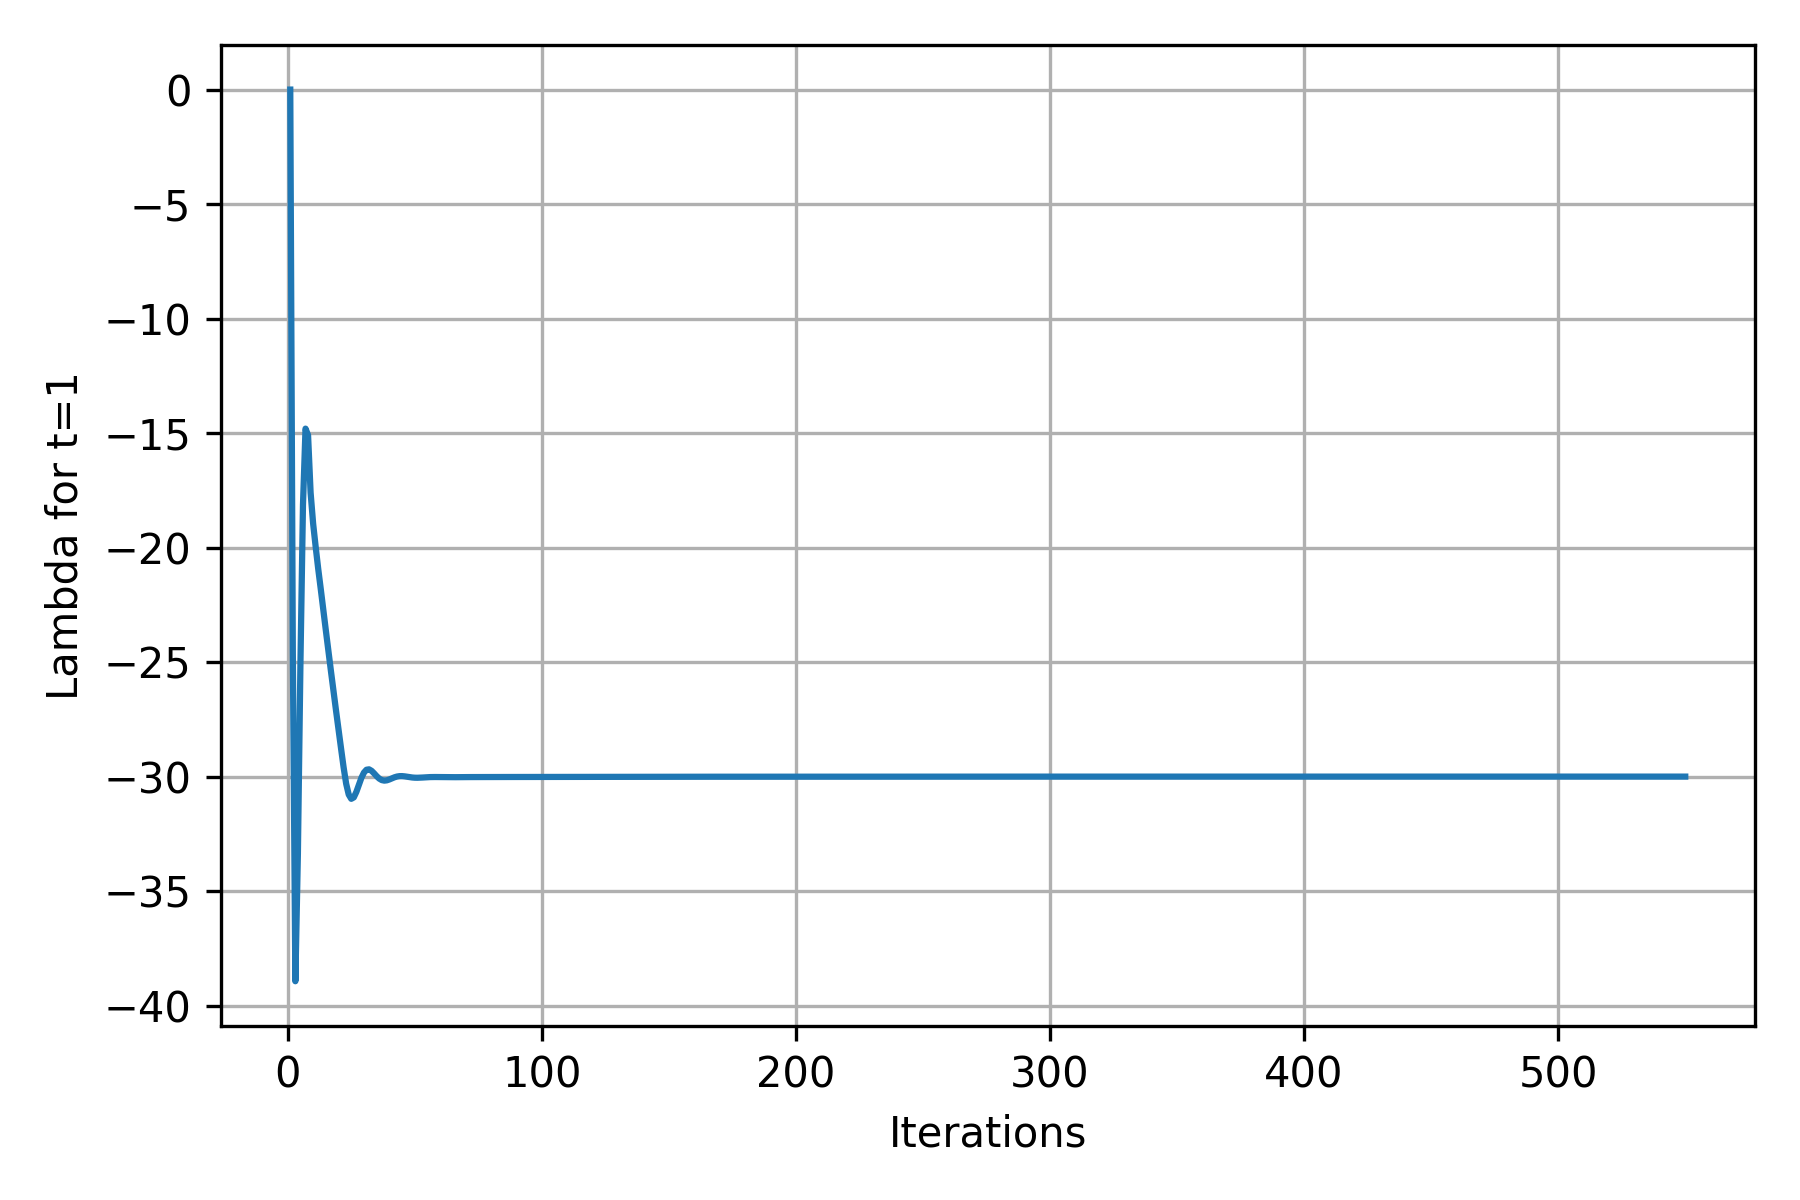
\includegraphics[width=0.8\textwidth]{plots/TNS_lambda_t1.png}
	\caption{Convergence Dual Variable $\lambda_1$}
	\label{fig:conv-lambda}
\end{figure}

After solving the convergence problem of the system balance dual variable, another divergence problem was faced. Although the correct value for $\lambda_t$ was found, the dual variables for the upper and lower power flow constraint did not converge. Figure (\ref{fig:conv-problem-2}) shows the convergence problem for $\rho_{2,1}$ at time step one for transmission line two. Remember that $\rho_{l,t}$ is the dual variable of the lower power flow constraint. If the demand is adapted so that no congestions occur, the dual variable converges. The same could be identified for the dual variable of the upper flow constraint $\mu_{l,t}$. Thus, it seemed that the algorithm could not handle transmission lines that were at their maximum line capacity. This led to the assumption that the penalty terms for the power flow constraints are not sensitive enough. \\

\begin{figure}[h!]
	\centering
	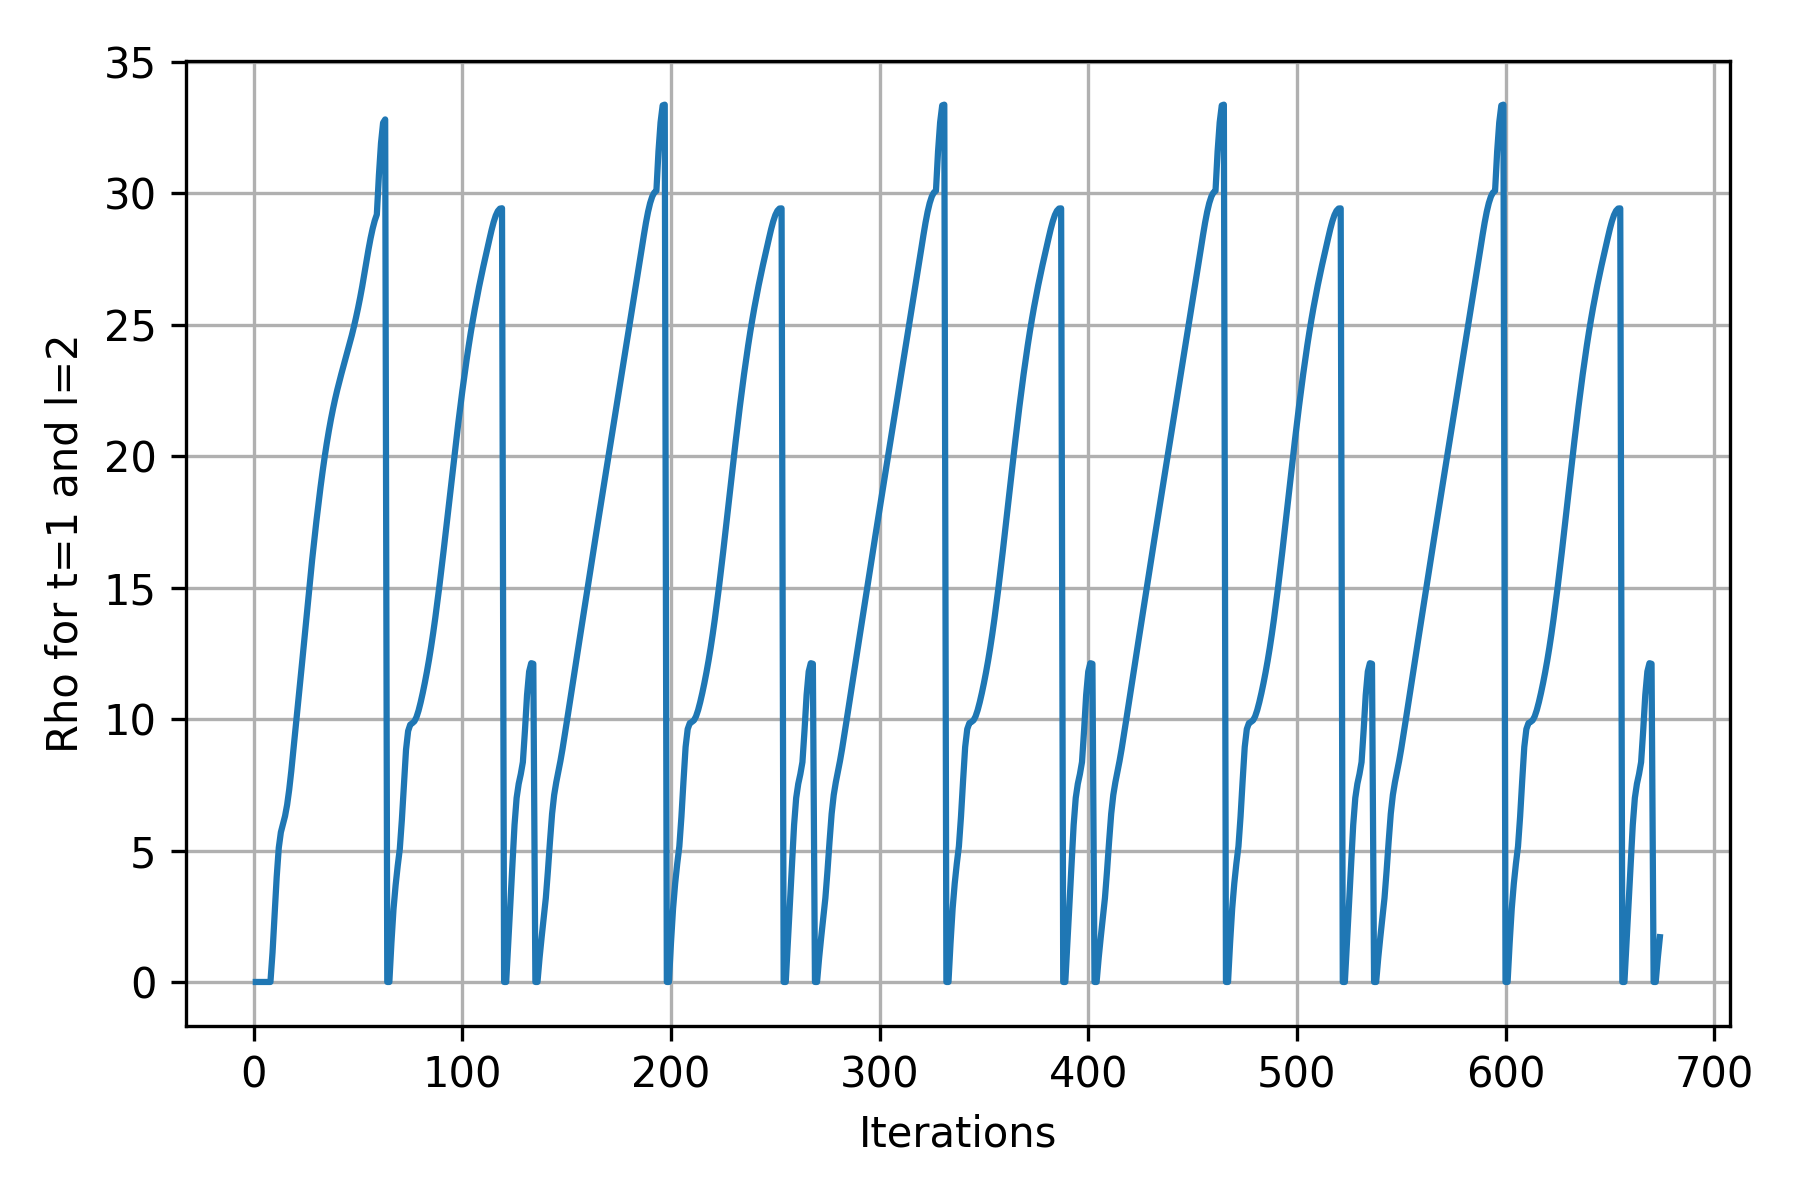
\includegraphics[width=0.8\textwidth]{plots/wrong_weight_rho_t1.png}
	\caption{Convergence Problem II: Wrong weight for power flow penalty term}
	\label{fig:conv-problem-2}
\end{figure}

Another observation supports this assumption. It was found that the value of the penalty terms of the power flow constraints is much smaller than the value of the penalty term of the system balance. Consequently, the weight in front of the power flow constraints was adapted to increase the influence of the power flow penalty terms. The general mathematical formulation of the \gls{admm} states that the relaxed complicated constraint is multiplied with the factor $\frac{\gamma}{2}$. This factor was adapted to a higher value to increase the impact of the power flow penalty terms. After several tries, the factor was changed to 10, as one can see in line \texttt{59} and \texttt{60} of listing (\ref{jl:sub-gen}), and the dual variables of the power flow constraints were not diverging anymore. \\

However, the algorithm was still not converging because the difference of the power flow dual variables between the current and the previous iteration was always greater than the defined threshold $\epsilon$. It was observed that the average slack variables $\Upsilon_{l,t}$ and $\Gamma_{l,t}$ were only almost zero for time steps and transmission lines that were at their maximum line capacity limit. In terms of the modeling framework, these average values should equal zero because the line capacity is fully utilized, see equations (\ref{eq:dom:con:pf-upper}) and (\ref{eq:dom:con:pf-lower}) for further reference. This was why the duals of the power flow constraint were not converging. As a solution, the update process of the power flow dual variables was adapted. The single elements of the average slack variables were checked against a certain threshold. If the values were smaller than the threshold, the corresponding entry of the dual variables is set to zero. Be aware that the mentioned threshold is not the threshold $\epsilon$ used for the convergence of the dual variables. One can find the implementation of the before mentioned process in lines \texttt{24} and \texttt{25} in listing (\ref{jl:update-all-duals}) that shows the update method for the upper flow dual variable $\mu_{l,t}$. Since this procedure is not very straightforward, it is explained with an example. At an iteration $i$ after solving all subproblems, the following average slack variable $\Upsilon_{l,t}$ for the upper power flow limit and dual variable $\mu_{l,t}$ was calculated:

\begin{equation}
	\Upsilon_{l,t} = \begin{bmatrix}
			30.00 & 6.70 \cdot 10^{-10} \\
			90.00 & 25.01 \\
			1.91 \cdot 10^{-8} & 69.98
		\end{bmatrix}
\end{equation}

\begin{equation}
	\mu_{l,t} = \begin{bmatrix}
			3.16 \cdot 10^{-6} & 129.89 \\
			7.31 \cdot 10^{-6} & 2.47 \cdot 10^{-5} \\
			25.46 & -9.86 \cdot 10^{-5}
		\end{bmatrix}
\end{equation}

The updated dual variable is then calculated with the help of equation (\ref{eq:update-duals:mu}). Since the entries for transmission line three and time step one and transmission line one and time step two are not zero, the updated dual is constantly increasing by a marginal value. Subsequently, the overall algorithm is not able to converge. Thus, the before-mentioned process is implemented. A boolean matrix is created that incorporates the check against the defined threshold of $10^{-2}$.

\begin{equation}
	\Upsilon_{l,t} < 10^{-2} = \begin{bmatrix}
			0 & 1 \\
			0 & 0 \\
			1 & 0
		\end{bmatrix}
\end{equation}

 This boolean matrix is then multiplied with the updated dual variable to smooth the values, see the following equation:
 
 \begin{equation}
	 \langle \begin{bmatrix}
			3.16 \cdot 10^{-6} & 129.89 \\
			7.31 \cdot 10^{-6} & 2.47 \cdot 10^{-5} \\
			25.46 & -9.86 \cdot 10^{-5}
	\end{bmatrix} \; , \; \begin{bmatrix}
			0 & 1 \\
			0 & 0 \\
			1 & 0
		\end{bmatrix} \rangle = \begin{bmatrix}
			0 & 129.89 \\
			0 & 0 \\
			25.46 & 0
		\end{bmatrix}
\end{equation}
 
 After implementing this correction, the dual variables of the power flow constraint were finally converging. Figure (\ref{fig:conv-mue}) and (\ref{fig:conv-rho}) show the convergence of the upper und lower power flow dual respectively. In figure (\ref{fig:conv-mue}), the line plot for transmission line one is not visible because it is covered by the line plot for transmission line two. Both transmission lines are not at their maximum line capacity limit. Thus the value of the dual variable is zero. The same applies to the line plots of transmission lines one and three in figure (\ref{fig:conv-rho}).

\begin{figure}[h!]
	\centering
	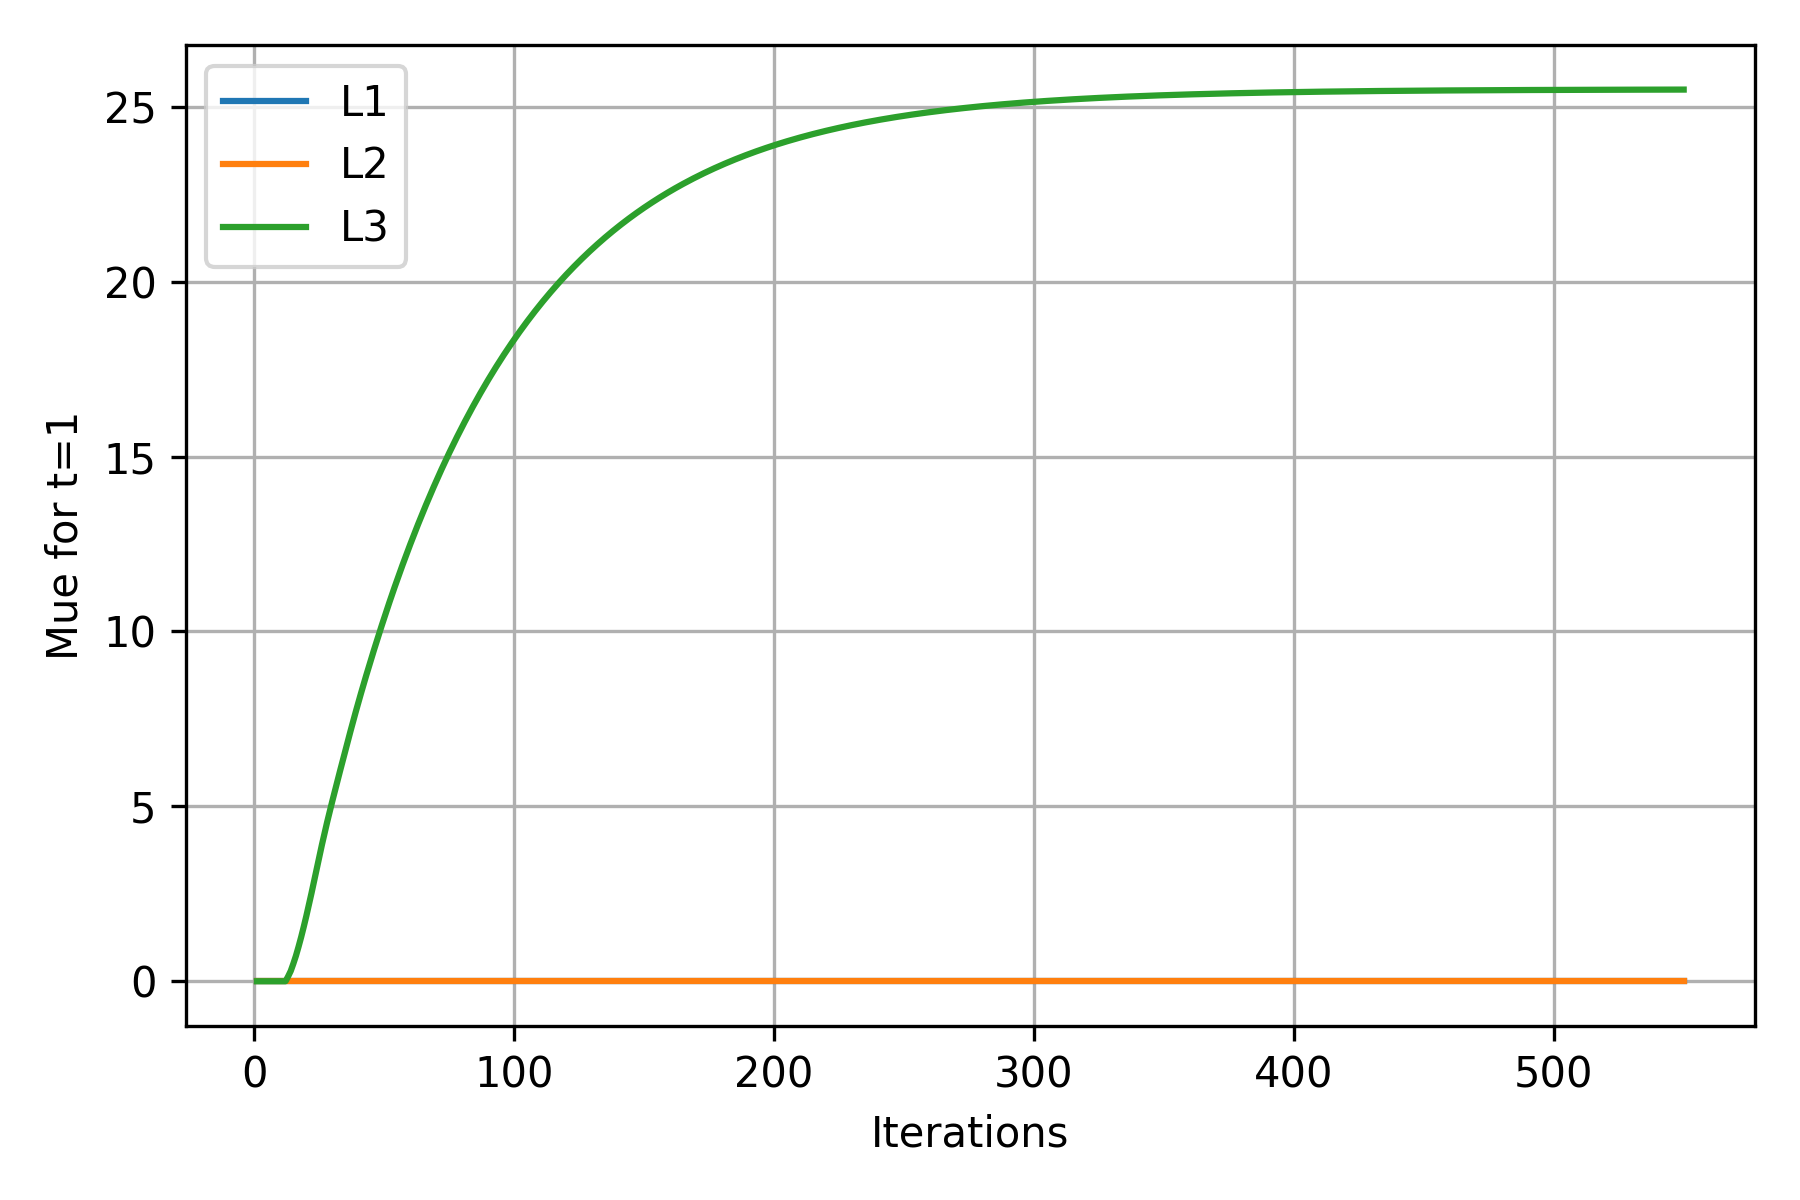
\includegraphics[width=0.8\textwidth]{plots/TNS_mue_t1.png}
	\caption{Convergence Dual Variable $\mu_{l,1}$}
	\label{fig:conv-mue}
\end{figure}

\begin{figure}[h!]
	\centering
	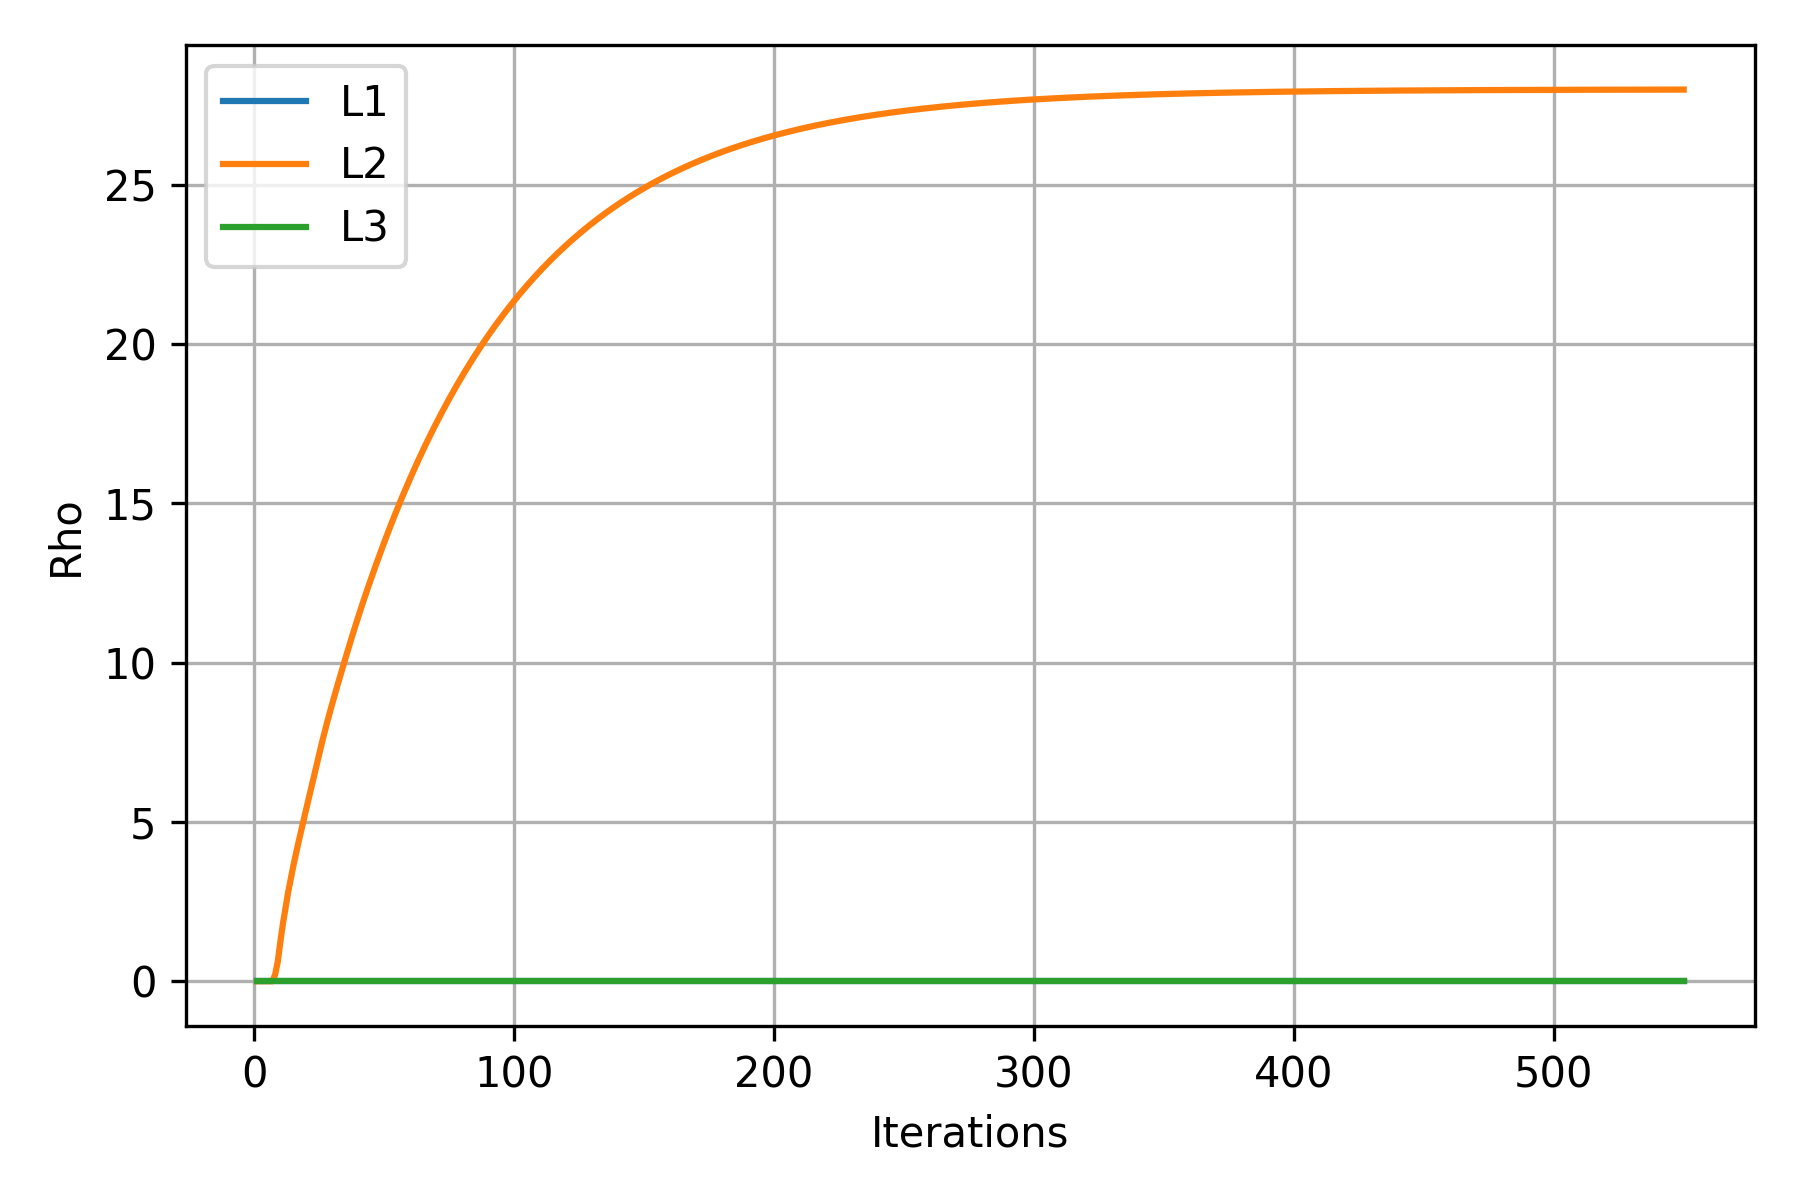
\includegraphics[width=0.8\textwidth]{plots/TNS_rho_t1.png}
	\caption{Convergence Dual Variable $\rho_{l,1}$}
	\label{fig:conv-rho}
\end{figure}


\subsection{Comparison between Centralized and Decentralized Approach}

The results for both the centralized optimal power flow and the decentralized optimal power flow were calculated for the \gls{tns}. For each network element, the obtained results are compared to each other. Tables are used to allow the reader to spot any differences quickly. First, the results of the generator elements are analyzed. \\

 \begin{table}[h!]
    \centering
    \begin{tabular}{p{0.2\textwidth}>{\centering\arraybackslash}p{0.2\textwidth}>{\centering\arraybackslash}p{0.2\textwidth}}
        \toprule
        \multirow{4}{*}{Generators $\set{G}$} & \multicolumn{2}{c}{Centralized OPF} \\
        {} & \multicolumn{2}{c}{\small{$P$ [MW]}} \\ 
        {} & {} & {} \\
        {} & $t=1$ & $t=2$ \\
        \midrule
        PV & 75.0000 & 80.0000 \\
        Wind & 110.0000 & 90.0000 \\
        Coal & 5.0000 & 220.0000 \\
        Gas & 0.0000 & 120.0000 \\
        \bottomrule
    \end{tabular}
    \caption{Generator results for centralized optimal power flow}
    \label{tab:res:cen-res-gen}
\end{table}

 \begin{table}[!h]
    \centering
    \begin{tabular}{p{0.2\textwidth}>{\centering\arraybackslash}p{0.2\textwidth}>{\centering\arraybackslash}p{0.2\textwidth}}
        \toprule
        \multirow{4}{*}{Generators $\set{G}$} & \multicolumn{2}{c}{Decentralized OPF} \\
        {} & \multicolumn{2}{c}{\small{$P$ [MW]}} \\ 
        {} & {} & {} \\
        {} & $t=1$ & $t=2$ \\
        \midrule
        PV & 75.0015 & 80.0000 \\
        Wind & 110.0008 & 90.0166 \\
        Coal & 4.9976 & 219.9834 \\
        Gas & 0.0000 & 120.0000 \\
        \bottomrule
    \end{tabular}
    \caption{Generator results for decentralized optimal power flow}
    \label{tab:res:dec-res-gen}
\end{table}

As one can see in tables \ref{tab:res:cen-res-gen} and \ref{tab:res:dec-res-gen}, there are only small differences between the results of both approaches. All of them are in the per mille range. The biggest difference can be observed for the wind generator at time step two. Here, the discrepancy is about 1.84 \textperthousand. Thus, one can state that the generator results of the decentralized optimal power flow resemble the results of the centralized approach. Furthermore, the generation results are as expected. The photovoltaic and wind generator are dispatched in both time steps since they are the cheapest generators in the system. The coal generator accounts for the residual in time step one due to the transmission line congestions. There is a surplus of 10 MW in time step one. This power is used to charge the battery storage, as one can see in the next two tables \ref{tab:res:cen-res-stor} and \ref{tab:res:dec-res-stor} that show the storage results for both approaches. \\

\begin{table}[!h]
    \centering
    \begin{tabular}{p{0.2\textwidth}>{\centering\arraybackslash}p{0.1\textwidth}>{\centering\arraybackslash}p{0.1\textwidth}>{\centering\arraybackslash}p{0.1\textwidth}>{\centering\arraybackslash}p{0.1\textwidth}>{\centering\arraybackslash}p{0.1\textwidth}>{\centering\arraybackslash}p{0.1\textwidth}}
        \toprule
        \multirow{4}{*}{Storages $\set{S}$} & \multicolumn{6}{c}{Centralized OPF} \\
        {} & \multicolumn{2}{c}{\small{$D$ [MW]}} & \multicolumn{2}{c}{\small{$C$ [MW]}} & \multicolumn{2}{c}{\small{$E$ [MWh]}} \\ 
        {} & {} & {} & {} & {} & {} & {} \\
        {} & $t=1$ & $t=2$ & $t=1$ & $t=2$ & $t=1$ & $t=2$ \\
        \midrule
        Battery & 0.0000 & 10.0000 & 10.0000 & 0.0000 & 10.0000 & 0.0000 \\
        \bottomrule
    \end{tabular}
    \caption{Storage results for centralized optimal power flow}
    \label{tab:res:cen-res-stor}
\end{table}

\begin{table}[!h]
    \centering
    \begin{tabular}{p{0.2\textwidth}>{\centering\arraybackslash}p{0.1\textwidth}>{\centering\arraybackslash}p{0.1\textwidth}>{\centering\arraybackslash}p{0.1\textwidth}>{\centering\arraybackslash}p{0.1\textwidth}>{\centering\arraybackslash}p{0.1\textwidth}>{\centering\arraybackslash}p{0.1\textwidth}}
        \toprule
        \multirow{4}{*}{Storages $\set{S}$} & \multicolumn{6}{c}{Decentralized OPF} \\
        {} & \multicolumn{2}{c}{\small{$D$ [MW]}} & \multicolumn{2}{c}{\small{$C$ [MW]}} & \multicolumn{2}{c}{\small{$E$ [MWh]}} \\ 
        {} & {} & {} & {} & {} & {} & {} \\
        {} & $t=1$ & $t=2$ & $t=1$ & $t=2$ & $t=1$ & $t=2$ \\
        \midrule
        Battery & 0.0000 & 10.0000 & 10.0000 & 0.0000 & 10.0000 & 0.0000 \\
        \bottomrule
    \end{tabular}
    \caption{Storage results for decentralized optimal power flow}
    \label{tab:res:dec-res-stor}
\end{table}

The tables above show the results of all storage-specific variables. This includes the discharge power, the charge power, and the energy level of all-time steps. The results of the centralized and decentralized approaches are the same. There are no differences in the per mille range. As expected, the storage is charged with the surplus of energy from the photovoltaic generator in time step one and discharged in time step two to reduce the total system costs by preventing the coal generator from producing more electricity. Hence, the battery's energy level is zero at the end of time step two. \\

Tables \ref{tab:res:cen-res-line} and \ref{tab:res:dec-res-line} list the results of all transmission lines in the system. Similar to the generator results, small differences between the centralized and decentralized approaches can be observed. However, most differences are only in the per mille range, with one exception. The discrepancy for line three at time step two is 0.0133 MW. Although this difference is a lot bigger than the difference from the generator results, it is still reasonable to claim that the transmission line results from the centralized approach equal the results from the decentralized approach. At time step one, transmission lines two and three are at their capacity limits. Transmission line two is at its lower limit of -45 MW, and transmission line three is at its upper limit of 70 MW. These congestions explain the observation that the coal generator is dispatched in time step one, although the cheaper photovoltaic and wind generator do not exploit their production limits. There is only one exploited transmission line at time step two. This is transmission line one at its upper limit with a utilization of 20 MW. At time step two, line three is not utilized at all because the wind and coal generator satisfy the nodal demand, respectively. \\

\begin{table}[!h]
    \centering
    \begin{tabular}{p{0.2\textwidth}>{\centering\arraybackslash}p{0.2\textwidth}>{\centering\arraybackslash}p{0.2\textwidth}}
        \toprule
        \multirow{4}{*}{Transmission Lines $\set{L}$} & \multicolumn{2}{c}{Centralized OPF} \\
        {} & \multicolumn{2}{c}{\small{Capacity [MW]}} \\ 
        {} & {} & {} \\
        {} & $t=1$ & $t=2$ \\
        \midrule
        Line 1 & -10.0000 & 20.0000 \\
        Line 2 & -45.0000 & 20.0000 \\
        Line 3 & 70.0000 & 0.0000 \\
        \bottomrule
    \end{tabular}
    \caption{Transmission line results for centralized optimal power flow}
    \label{tab:res:cen-res-line}
\end{table}

\begin{table}[!h]
    \centering
    \begin{tabular}{p{0.2\textwidth}>{\centering\arraybackslash}p{0.2\textwidth}>{\centering\arraybackslash}p{0.2\textwidth}}
        \toprule
        \multirow{4}{*}{Transmission Lines $\set{L}$} & \multicolumn{2}{c}{Decentralized OPF} \\
        {} & \multicolumn{2}{c}{\small{Capacity [MW]}} \\ 
        {} & {} & {} \\
        {} & $t=1$ & $t=2$ \\
        \midrule
        Line 1 & -10.0005 & 20.0033 \\
        Line 2 & -45.0011 & 19.9967 \\
        Line 3 & 70.0013 & 0.0133 \\
        \bottomrule
    \end{tabular}
    \caption{Transmission line results for decentralized optimal power flow}
    \label{tab:res:dec-res-line}
\end{table}

Tables \ref{tab:res:cen-res-node} and \ref{tab:res:dec-res-node} show the injections at each system node. Once again, the differences between the centralized and decentralized approaches are minimal. The biggest discrepancy can be observed at nodes two and three for time step two. The difference between the two approaches is here 8.3 \textperthousand. Subsequently, the claim that both approaches yield the same results is still valid. The results for the nodal injections are as expected. At time step one, node three is the only node that imports electricity from the other nodes. It is the other way around for time step one, where only node one imports electricity from the other nodes. The sum of all nodal injections equals zero for every time step. Thus, the system balance constraint is ensured. \\

\begin{table}[!h]
    \centering
    \begin{tabular}{p{0.2\textwidth}>{\centering\arraybackslash}p{0.2\textwidth}>{\centering\arraybackslash}p{0.2\textwidth}}
        \toprule
        \multirow{4}{*}{Nodes $\set{N}$} & \multicolumn{2}{c}{Centralized OPF} \\
        {} & \multicolumn{2}{c}{\small{Injection [MW]}} \\ 
        {} & {} & {} \\
        {} & $t=1$ & $t=2$ \\
        \midrule
        Node 1 & 55.0000 & -40.0000 \\
        Node 2 & 60.0000 & 20.0000 \\
        Node 3 & -115.0000 & 20.0000 \\
        \bottomrule
    \end{tabular}
    \caption{Node results for centralized optimal power flow}
    \label{tab:res:cen-res-node}
\end{table}

\begin{table}[!h]
    \centering
    \begin{tabular}{p{0.2\textwidth}>{\centering\arraybackslash}p{0.2\textwidth}>{\centering\arraybackslash}p{0.2\textwidth}}
        \toprule
        \multirow{4}{*}{Nodes $\set{N}$} & \multicolumn{2}{c}{Decentralized OPF} \\
        {} & \multicolumn{2}{c}{\small{Injection [MW]}} \\ 
        {} & {} & {} \\
        {} & $t=1$ & $t=2$ \\
        \midrule
        Node 1 & 55.0015 & -40.0000 \\
        Node 2 & 60.0008 & 20.0166 \\
        Node 3 & -115.0020 & 19.9834 \\
        \bottomrule
    \end{tabular}
    \caption{Node results for decentralized optimal power flow}
    \label{tab:res:dec-res-node}
\end{table}

\begin{table}[!h]
    \centering
    \begin{tabular}{p{0.2\textwidth}>{\centering\arraybackslash}p{0.2\textwidth}>{\centering\arraybackslash}p{0.2\textwidth}}
        \toprule
        \multirow{4}{*}{} & \multicolumn{2}{c}{Decentralized OPF} \\
        {} & \multicolumn{2}{c}{\small{Price [EUR]}} \\ 
        {} & {} & {} \\
        {} & $t=1$ & $t=2$ \\
        \midrule
        System & 30.0000 & 30.0000 \\
        Node 1 & 36.6000 & 82.0000 \\
        Node 2 & 15.2000 & 4.0000 \\
        Node 3 & 30.0000 & 30.0000 \\
        \bottomrule
    \end{tabular}
    \caption{Prices for the centralized optimal power flow}
    \label{tab:res:cen-res-prices}
\end{table} 

\begin{table}[!h]
    \centering
    \begin{tabular}{p{0.2\textwidth}>{\centering\arraybackslash}p{0.2\textwidth}>{\centering\arraybackslash}p{0.2\textwidth}}
        \toprule
        \multirow{4}{*}{} & \multicolumn{2}{c}{Decentralized OPF} \\
        {} & \multicolumn{2}{c}{\small{Price [EUR]}} \\ 
        {} & {} & {} \\
        {} & $t=1$ & $t=2$ \\
        \midrule
        System & -30.0000 & -30.0004 \\
        Node 1 & -36.5972 & -81.9756 \\
        Node 2 & -15.2162 & -4.0127 \\
        Node 3 & -30.0000 & -30.0004 \\
        \bottomrule
    \end{tabular}
    \caption{Prices for the decentralized optimal power flow}
    \label{tab:res:dec-res-prices}
\end{table}

Next, the system electricity price and the nodal prices are analyzed. The system electricity price is the dual variable of the system balance constraint. According to \citet{yang2019}, the nodal price can be calculated as the sum of the system price and the dual variables of the upper and lower power flow constraint. The corresponding mathematical formulation can be found in equation (\ref{eq:nodal-prices}).

\begin{equation}
	r_{n,t} = \lambda_t + \sum_{l \in \set{L}} (\mu_{l,t} + \rho_{l,t}) * PTDF_{l,n}
	\label{eq:nodal-prices}
\end{equation}

Retrieving the dual variable of the system balance and calculating the nodal prices for each time step with the help of equation (\ref{eq:nodal-prices}) yields the results that are shown in tables \ref{tab:res:cen-res-prices} and \ref{tab:res:dec-res-prices}. The absolute prices are nearly the same. However, the algebraic sign is different. The reason here is the way the system balance is formulated in section \ref{sec:app:dom} and how the decentralized algorithm is set up. Thus, the algebraic sign is irrelevant and can be ignored for this analysis. The differences between the two approaches are again only marginal. Although the differences are more significant than the generator results, it is possible to claim that the two approaches yield the same system and nodal prices for every time step. The interpretation of the prices is not straightforward because of the power line congestion. However, the prices are like one would assume. The most significant nodal price (82 EUR) is at node one for time step two, where we have the highest congestion in the network. This leads to the dispatch of the gas generator, which is the most expensive generator. The cheapest nodal price (4 EUR) is at node two for time step two.

